\label{section:motivationBank}

We now consider as an example a simplified banking application.   \sd{Assume a module (a repository of class code) say, $\M_{BA}$,  with classes \prg{Bank}, \prg{Account} and possibly some more classes. In the diagram below we depict objects through rounded boxes, and the contents of fields through arrows. }%consisting of a \prg{Bank} object at \prg{1},
%and three \prg{Account} objects at \prg{2}, \prg{3} and \prg{4}.}

 \begin{tabular}{ll}
 \begin{minipage}{0.49\textwidth}
\sd{We use the transparent green rectangle to show which objects belong to  $\M_{BA}$. 
We have a  \prg{Bank} object at \prg{1},
 three \prg{Account} objects at \prg{2}, \prg{3} and \prg{4}, and some further  objects of the 
   module $\M_{BA}$  %\prg{Bank}/\prg{Account} module are depicted in 
at \prg{7}, \prg{8} \etc, all in green. 
The objects
outside the module are depicted in grey; here objects \prg{100}, \prg{101}, \prg{200}, and \prg{201}.}
 \end{minipage}
 &
 \begin{minipage}{0.45\textwidth}
 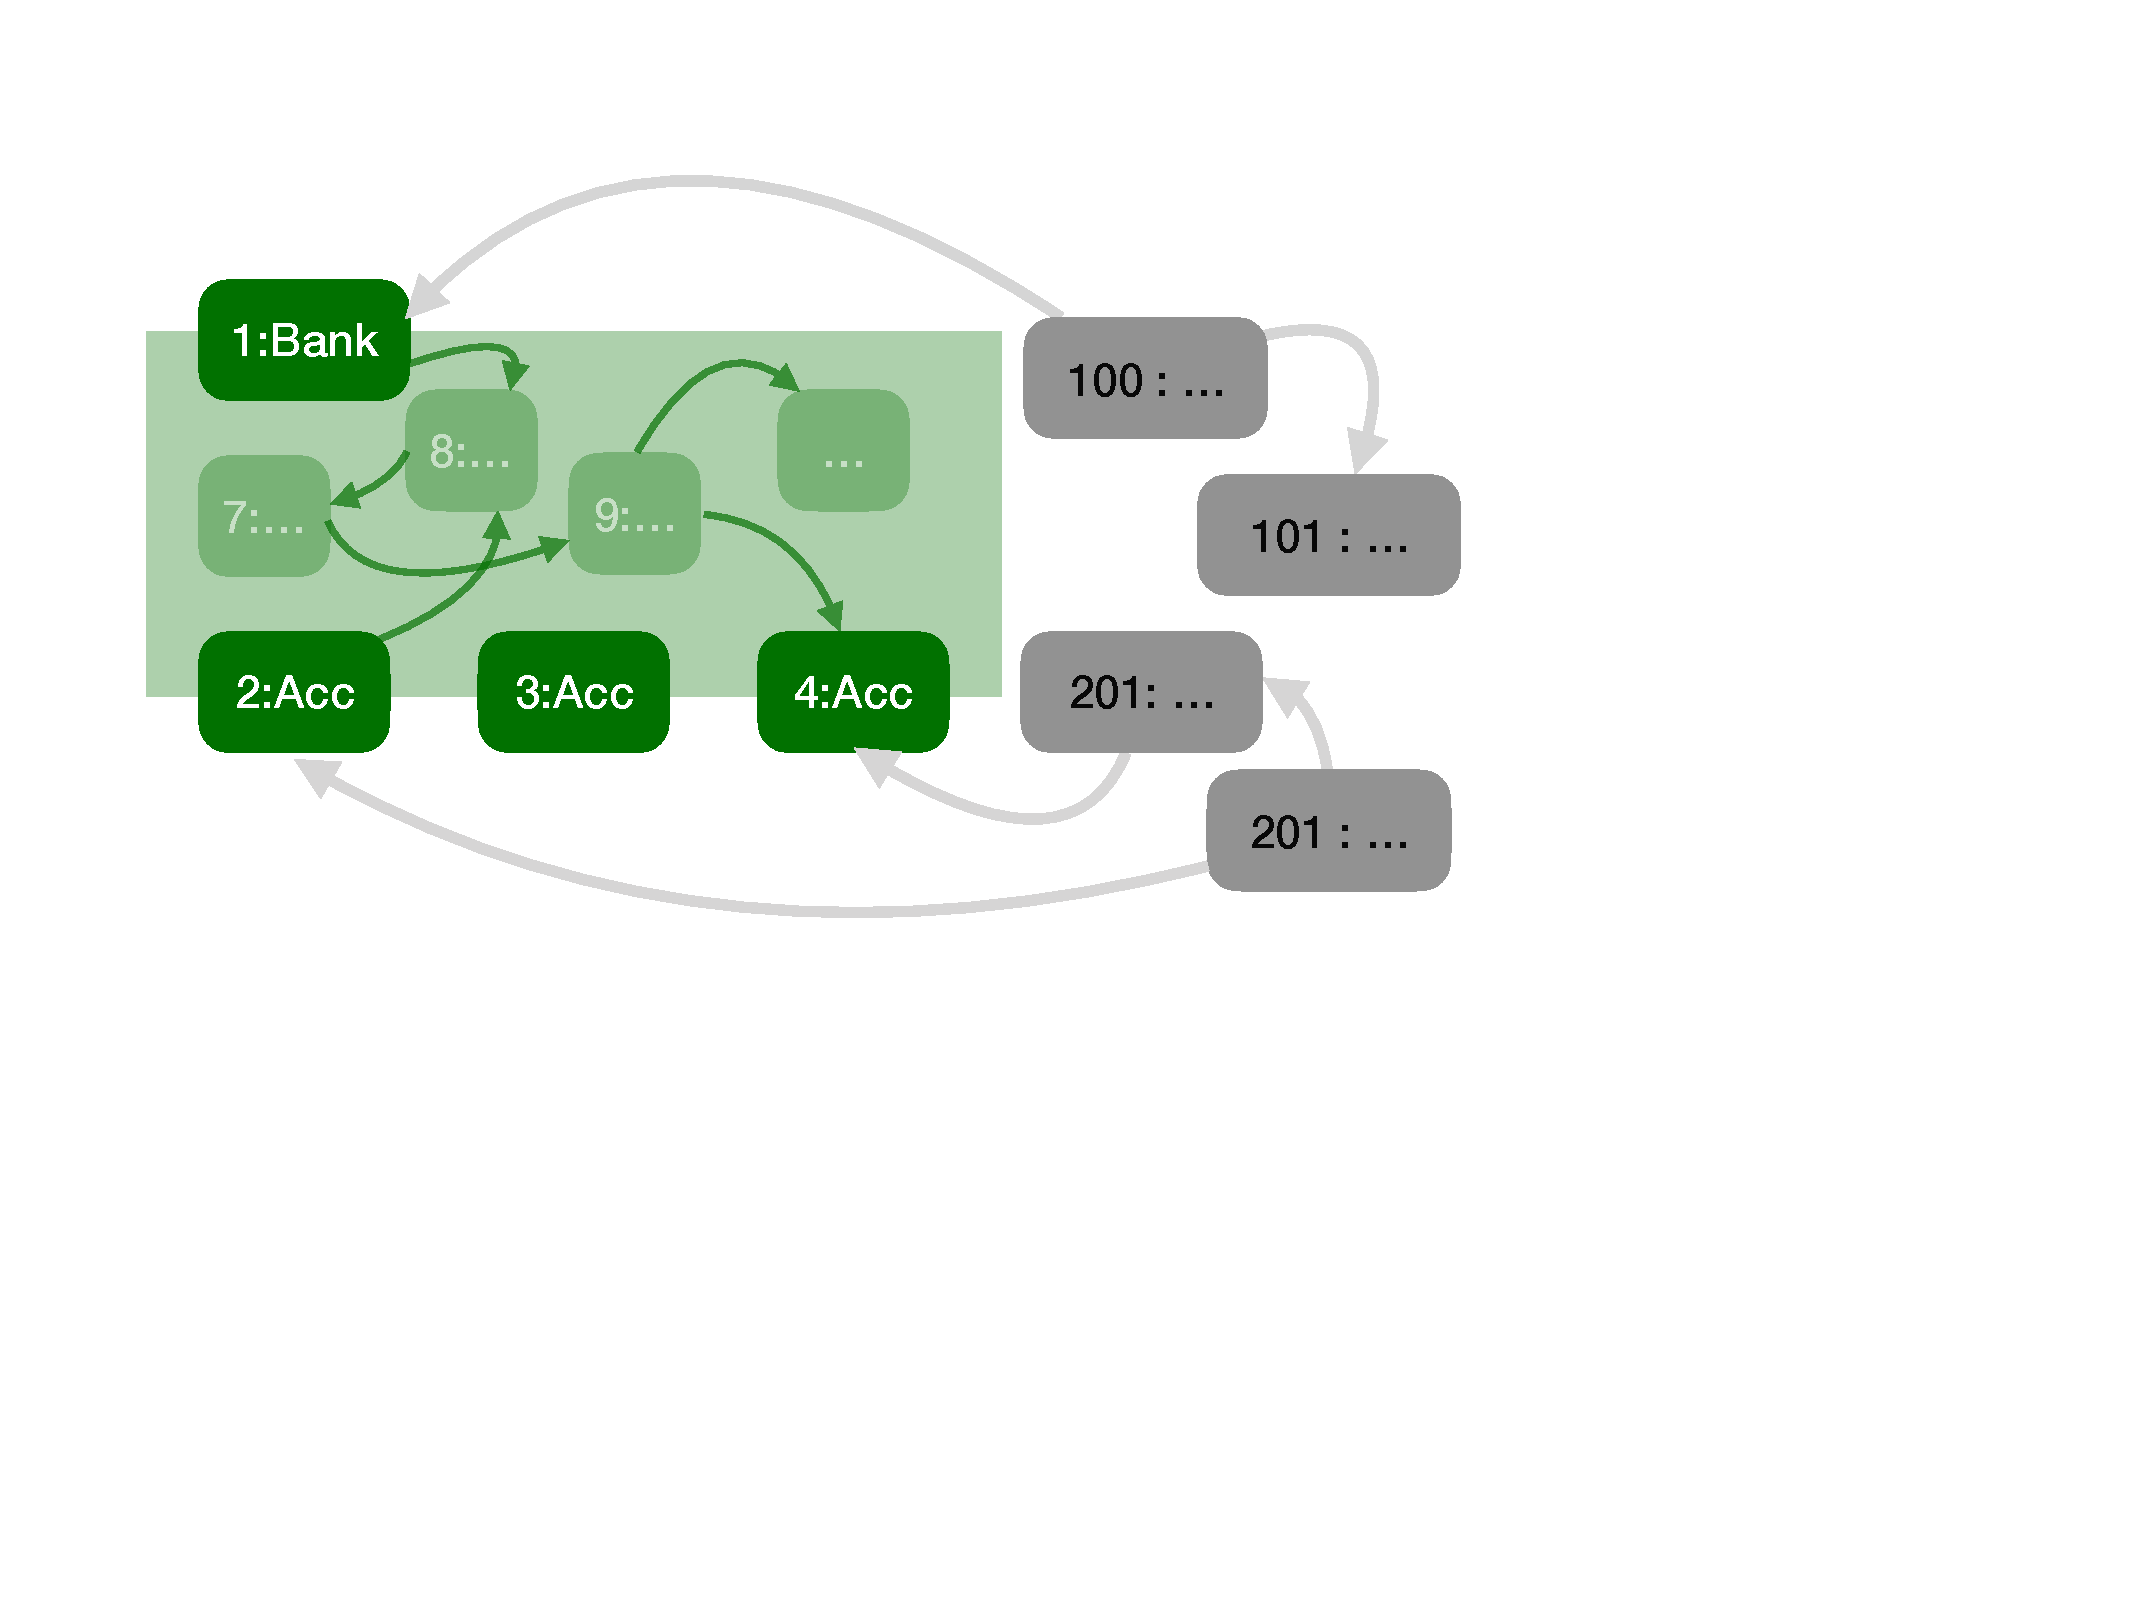
\includegraphics[width=\linewidth, trim=85  330 300 70,clip]{diagrams/BankAccount_With_Internal.pdf}
%% x y z w
%% x eats space from left, if you increase it the diagram decreases from left
%% y seems to eat up the bollom
%% z takes from right
%% w eats space from top, if you increase it the diagram decreases from top
 \end{minipage}
\end{tabular}

\sdcomment{After discussion with Susan I think we need such a diagram. But the flow with the next para is nit good.}

Traditional functional specifications describe what components are
guaranteed to do. So long as a method is called in a state satisfying
its preconditions, the method will complete its work and establish a
state satisfying its postconditions.  
\sd{Thus, the pre-condition and the method call together form a \emph{sufficient}
condition for the nethod's effect.}
% Method specifications thus
% define the \textit{sufficient} conditions for their methods' behaviour
% to be invoked.


Consider the specification of a trivial Bank component in
fig.~\ref{fig:BankSpec}.  The bank is essentially a wrapper for a map
from account objects to account balances: given an instance of a Bank
component, calling \prg{newAccount} returns a new account object with
an initial balance. 
\sdcomment{ \kjx{changed it so it behaves more like a
bank, rather an a currency:  you open an account with a new balance.
We can no longer talk about the preservation of a currency,
but the amount in the bank must be the sum of arguments to newAccount.}
I think thag s exactly what currency is. The Bank here is no different than the Mint.}

Given an account, calling \prg{balance} with an
account returns the account balance, and calling \prg{deposit} with
two accounts deposits funds from the source to the destination account.
\sdcomment{\se{I am very confused about deposit. If sb and db can be the same bank, 
\sd{se and sb are numbers in the spec} then the statements to ensure that {\tt{steal}} cannot be included in the system (that is only one account is changed) won't hold. If they must be different as is in the Chainmail spec, it is a very peculiar bank where one cannot transfer money between two accounts in the same bank. I also am unclear about the changes to an account caused by a deposit to another account. Perhaps my difficulty comes from the policy deposit where sb and db are of equal weight whereas the Chainmail spec has the client in sb calling deposit on the player in db and it can only do so if it knows db's account number.}}
\sdcomment{Perhaps we should inline Fig. 3 and 4? Also, do we need both specification and policy? We do not have
such syntax in this paper.}

\begin{figure}[tbp]
\begin{lstlisting}
  specification Bank {

    ghost field ledger : Map[Account, Number]

    policy newAccount {
        a : Account, b : Bank, n : Number
          { def a ;= b.newAccount(n) }
        FRESH(a) & ledger.containsKey(a)
    }

    policy balance {
      a : Account, b : Bank, n : Number
        { n := b.balance(a) }
      n == ledger.at( a )
    }

    policy deposit {
      src, dst : Account, b : Bank, sb, db, n : Number
      sb == ledger.at(src), db == ledger.at(dst), n > 0, src=/=dst
        { b.deposit(dst, src, n) }
      ledger.at(src) == sb - n
      ledger.at(dst) == db + n
    }
  }
\end{lstlisting}
\kjx{will update style sometime}\sd{to add: FRESH(a) AND ledger.containsKey(a) AND  ledger.at(a)=n  AND a:Account }
\caption{Functional specification of a Bank}
\label{fig:BankSpec}
\end{figure}

\sdcomment{"Map" should be a mathematical construction, not some more syntax. And why does "at" mean lookup}
\secomment{Why not "dst.deposit(src,n)" instead.}
\secomment{The name "deposit" is confusing because it depostis into dst, but withdraws from the argument.}
\secomment{Make clear in the spec-s above what is the PRE-condition and what is the POST-condition.}



The specification in fig.~\ref{fig:BankSpec} is enough to let us
calculate the result of operations on the bank and the accounts ---
for example it is straightforward to determine that the code in
fig.~\ref{fig:rego} satisfies its assertions: given that the
\prg{acm} object has a balance of 10,000 before an author is
registered then afterwards it will have a balance of 11,000 while the
\prg{author} now has a balance of 500 from a starting balance of 1,500
(barely enough to buy a round of drinks at the conference hotel bar).


\begin{figure}[tbp]
\begin{lstlisting}
  assume b.balance(acm) == 10000
  assume b.balance(author) == 1500

  b.deposit(acm, author, 1000)

  assert b.balance(acm) == 11000
  assert b.balance(author) == 500
\end{lstlisting}
\caption{Registering at a Conference}
\label{fig:rego}
\end{figure}


This reasoning is fine in a closed world, where we only have to
consider complete programs, where all the code in our programs (or any
other systems with which they interact) is under our control.   In an
open world, however, things are more complex: our systems will be made
up of a range of components, many of which we do not control; and
furthermore will have to interact with external systems which we
certainly do not control.  Returning to our author, say some time
after registering by executing the code in fig.~\ref{fig:rego}, they
attempt to pay for a round at the bar.  Under what circumstances can
they be sure they have enough funds in their account?

To see the problem, consider the additional function specified in
fig.~\ref{fig:steal}. This method says the bank additionally provides a
\prg{steal} method that empties out every account in the bank and puts
all their funds into the thief's account. If this method exists, and
if it is somehow called between registering at the conference and
going to the bar, the author (actually everyone using the same bank)
will find all their accounts empty (except the thief, of course).

\begin{figure}[tbp]
\begin{lstlisting}
  specification Theft {

    policy steal {
      b : Bank, thief in Account, m in Map[Account, Number]
      m == b.ledger
        { b.steal(thief) }
      forall a in dom(m) :
        ledger.at(a) =
          if (a == thief) then {sum(codom(m))} else 0
    }
  }
\end{lstlisting}
\caption{Sufficient Specification of Theft}
\label{fig:steal}
\end{figure}

The critical problem is that a bank implementation including a \prg{steal}
method would meet the functional specifications of the bank from
fig.~\ref{fig:BankSpec}, so long as its \prg{newAccount},
\prg{balance}, and \prg{deposit} methods do meet
that specification.

One obvious solution would be to return to a closed-world
interpretation of specifications: we interpret specifications such as
fig.~\ref{fig:BankSpec} as \emph{exact} in the sense that only
implementations that meet the functional specification exactly,
\emph{with no extra methods or behavour}, are considered as suitable
implementations of the functional specification. The problem is that
this solution is far too strong: it would for example rule out a bank
that simply counted the number of deposits that had taken place,
i.e. met fig.~\ref{fig:count} as well as fig.~\ref{fig:BankSpec}.

\begin{figure}[tbp]
\begin{lstlisting}
  specification CountDeposits {

    ghost field count : Number = 0

    policy deposit {
      c : Number = count
        { b.deposit(dst, src, n) }
      count == c + 1
    }

    policy count {
      b : Bank
        { c = b.countDeposits }
      c == b.count
    }
  }
\end{lstlisting}
\caption{Functional specification counting the number of deposits}
\label{fig:count}
\end{figure}


What we need is some way to permit bank implementations that meet
fig.~\ref{fig:count} but to forbid implementations that meet fig.~\ref{fig:steal}.  
The key here is to capture the (implicit)
assumptions underlying fig.~\ref{fig:BankSpec}, and to provide
additional specifications that capture those assumptions.  There are
at least two assumptions that can prevent methods like \prg{steal}:

\begin{enumerate}
\item after creation, the \emph{only} way an account's
  balance can be changed is if a client   calls the \prg{deposit} method \sd{with the
  account as the receiver or as an argument}
\item an account's balance can \emph{only} be changed if a client has
  that particular account object.
\end{enumerate}

Compared with the functional specification we have seen so far, these
assumptions capture \emph{necessary} conditions rather than
\emph{sufficient} conditions. It is necessary that the \prg{deposit}
method is called to change an account's balance, and it is necessary
that the particular account object can be passed as a parameter to
that method. The fig.~\ref{fig:steal} specification is not consistent
with these assumptions, while the.~\ref{fig:count} specification is
consistent with these assumptions.

\sdcomment{Chopped this as I believe we have said earlier:
\kjx{\textbf{NEED TO DECIDE ON CONTRIBUTIONS.
The contribution of this paper is a specification langauge and
semantics that can be used to specify necessary specifications, and a
semantics for those specifications that can determine whether some
functional (sufficient) specifications are consistent (or not) with
the necessary specifications. }}Also think that we do not do
"can determine whether some
functional (sufficient) specifications are consistent (or not) with
the necessary specifications."}

%Fig.~\ref{fig:nec} shows how we
%can 
\sd{Below we} express these two informal \sd{requirements} %assumptions using 
in \Chainmail.  Rather than %specifying \prg{functions} to  describe
\sd{specifying} the behaviour of particular methods when they are called, we
write policies \sdcomment{Not using \prg{policies}, as we have no synatx for these}  that range across the entire behaviour of the
component.
\vspace{.2cm}

%\begin{figure}[htbp]
%%\begin{definition}
%\label{def:pol2}

(1)\ \  $\triangleq$\ \ $\forall \prg{a}:\prg{Account}\ [\ \ \ \  \Changes{\prg{a.balance}}  \ \    
    \longrightarrow \ \    \hfill$ \\
  $\strut \hspace{2.3cm} 
% \exists \prg{o}.\ [\ \External{\prg{o}} \ \wedge \  \Past{\Calls{\prg{o},\prg{deposit},\_,\_}}   \  \ ] \ \  \ \ ]$
% External holds implcitlyy
 \exists \prg{o}. [\  \Past{\Calls{\prg{o},\prg{deposit},\prg{a},\_,\_}}\ \vee\  \Past{\Calls{\prg{o},\prg{deposit},\_,\prg{a},\_}} \ ] \ \ ] \hfill $

\vspace{.4cm}

    (2)\ \  $\triangleq$\ \ $\forall \prg{a}:\prg{Account}\ .\forall \prg{S}:\prg{Set}.\ [  \ \Using{(\Future{\,\Changes{\prg{a.balance}}})\,}{\prg{S}\,}\ \ \   \
    \longrightarrow$ \\
 $\strut \hspace{3.9cm} \hfill \exists \prg{o}.\ [\, \prg{o}\in \prg{S}\ \wedge \ \CanAccess{\prg{o}}{\prg{a}}\ \wedge  \  \External{\prg{o}}  \ ] \ \ \ \ ]$

%\end{definition}
%\vspace{-.2cm}
%\caption{Necessary specifications for \prg{deposit}}
%%\label{fig:nec}
% \end{figure}
\vspace{.2cm}

\sdcomment{We have to explain that the two objects above may be different .}
 
Policy (1) %in fig.~\ref{fig:nec} says 
says that if   an account's balance is changed
($\Changes{\prg{a.balance}}$)
then there must be some client object \prg{o}
that in the past (${\Past{...}}$) called the \prg{deposit} method with \prg{a} as a receiver or an an argument ($\Calls{\prg{o,deposit,\_,\_}}$).
\sdcomment{ We no longer need "which is outside the
bank and its associated accounts ($\prg{o} \notin\prg{Internal}(\prg{a})$)" -- and I have chopped it from
the spec. This is because of the visible states :-)}
\sdcomment{ I propose that we change deposit so that it is called on the account object.}

Policy (2) similarly constrains any possible change to an 
account's balance: 
If at some future point the balance changes   (${\Future{...}}$) %(${\Future{\,\Changes{...}}}}$), 
and if the footprint of the
execution that brings about this change is the set of objects in \prg{S} (\ie $\Using{...}{\prg{S}}$), then 
at least one of these objects (\prg{o}) has (direct) access to that account object
($\CanAccess{\prg{o}}{\prg{a}}$).
 \sdcomment{chopped "but requires that the client object making the call
has direct access" because a) the spec did not say it, and b) it is not the case.}


A \sd{holistic} specification for the bank account, then,
would be our original sufficient functional specification from
fig.~\ref{fig:BankSpec} plus the necessary security policy
specification in fig.~\ref{fig:nec}.   \sd{We swill discuss the meaning of the
policies in more detail in the next section. }\sdcomment{Where shall we say this?}
This holistic specification
permits an implementation of the bank that also meets the \prg{count}
specification from fig.~\ref{fig:count}, but does not permit an
implementation that also meets the \prg{steal} specification from
fig.~\ref{fig:steal}.

\sdcomment{We no longer need this=/=a}



\begin{figure}[tbp]
\begin{lstlisting}[escapeinside=`']
  specification Robust-Bank {

    policy call-deposit {
      `$\forall$' a : Account, S : Footprint
         this != a `$\wedge \Using{(\Future\Changes{\prg{a.balance}})}{\prg{S}}\ \ \ \longrightarrow$'
             `$\exists \prg{o}.\ [\, \prg{o}\in \prg{S}\ \wedge \ \Calls{\prg{deposit}}\ \wedge  \ \prg{o} \notin\prg{Internal}(\prg{a}) \ ]$'  
    }

    policy access-account {
      `$\forall$' a : Account, S : Footprint
         this != a `$\wedge \Using{(\Future\Changes{\prg{a.balance}})}{\prg{S}}\ \ \ \longrightarrow$'
             `$\exists \prg{o}.\ [\, \prg{o}\in \prg{S}\ \wedge \ \CanAccess{\prg{o}}{\prg{a}}\ \wedge  \ \prg{o} \notin\prg{Internal}(\prg{a}) \ ] \ \ \ \ ]$'
    }
  }
\end{lstlisting}
\caption{Necessary specifications for \prg{deposit} -- James version}
\label{fig:kjx}
\end{figure}




\sdcomment{\se{I think your necessary conditions don't really tally with what happens with banks. In banks you can transfer to an account that you know nothing about, just by giving a bank account number, \sd{I think that what we call Account here is the account number, but we should perhaps clarify} so I don't see the purpose of the access rule. Also you can transfer within a bank and it is a null action but you usually can transfer money to yourself. The thing you usually can't do is transfer more money than you have in the account, but that would be more code in deposit so I understand why it is omitted. I can see from Chainmail why you wish to have rule 2, but as your bank differs from a real bank you should describe this very simple bank so that people don't have a real bank in their heads when reading your policies.}}

We can then prove that e.g.\ the \prg{steal} method from
fig.~\ref{fig:steal} is inconsistent with both of these policies.
First, the \prg{steal} method clearly changes the balance of
every account in the bank, but policy (1) requires that any method
that changes the balance of any account must be called \prg{deposit}.
Second, the \prg{steal} method changes the balance of every account in
the system, and will do so without the called having a reference to
most of those accounts, which breaches policy (2).   Note
that \prg{steal} putting all the funds into the thief's account
does not breach policy (2) with respect to the thief's own account,
because that account is passed in as a parameter to the \prg{steal}
method, and so the called of the \prg{steal} must have access to that
account.


\paragraph{random minor point}

These necessary specification policies
can be defined and interpreted independently of any particular
implementation of a specification --- rather our policies constrain
implementations, in just the same way as traditional functional
specifications.  This is in contrast to e.g.\ class invariants, which
establish invariants across the implementation of an abstract, or
abstraction functions, which link an abstract model to a concrete
implementation of that model. 
